\section{Working with GTFS data}
\label{sec:gtfs}

GTFS (general transit feed specification)
is an API (application programming interface) specification for transit data
detailing it should be organised,
making access easier for application developers.
Developed and maintained by Google \citep{GoogleDevelopers_2006},
who make use of it in their Google Maps Transit Directions,
it is used by over 900~transit providers around the world,
including here in Auckland, New Zealand
(source \url{http://transitfeeds.com}).
An advantage of this for us is that,
provided our application depends solely on GTFS data,
after developing it locally in Auckland it can be deployed to any other GTFS-based
public transport system with minimal modification.


There are two components to GTFS.
The first, \emph{GTFS static}, includes information about stops, routes, trips, and shapes:
a \emph{stop} is a physical location where passengers can embark and disembark the vehicle;
a \emph{route} is a sequence of two or more stops displayed as a single service;
a \emph{trip} is an instance of a route occuring at a specific time of day; and
a \emph{shape} is the sequence of points defining a vehicle's path along a route
\citep{GoogleDevelopers_2006}.
The second component is \emph{GTFS realtime},
which is only available in a subset of the providers due to the requirement of 
onboard GPS and a central server.
It provides a standardised format for sharing vehicle positions and trip delays,
which are often accessed via an API which developers can use in \rt applications.


Before we can develop our application,
we need to modify the raw GTFS information to make it possible to detect common roads.


\subsection{Transit network construction}
\label{sec:network_build}

Arguably one of the most important predictors of arrival time is
the travel time along intermediate roads,
however in most applications this vital information is unavailable,
at least directly. 
Several predictive approaches using \emph{headway},
the time between consecutive trips along the same route,
have been proposed \citep{Hans_2015};
however, while this is reasonable for high frequency routes,
low frequncy routes will be unable to react quickly to changes in congestion,
and it is for these routes which reliable ETAs are arguably more important,
since the cost of missing a bus is greater.


One solution would be to use information obtained from
vehicles servicing other routes but traveling along the same roads
to estimate arrival times.
The simplest method of identifying overlapping routes is to compare
the stop sequence: 
routes with a common sub-sequence of stops must be traveling the same route between them.
While there are several exceptions, for example express routes 
and multi-stop locations where there are high numbers of routes,
it is a viable enough simplication for the purposes of this paper.
Figure~\ref{fig:network_creation} demonstrates how several overlapping routes 
are merged to form a road network.
In section~\ref{sec:kf} we present a model for estimating vehicle travel time
along a road segment.

\begin{figure}[tb]
    \centering
    \begin{subfigure}{0.7\textwidth}
        \centering
        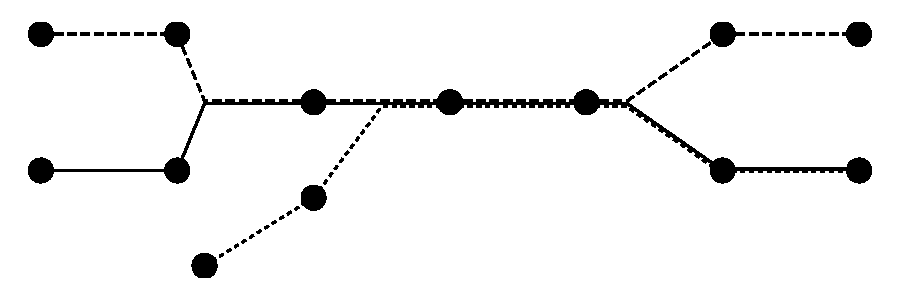
\includegraphics[width=0.95\textwidth]{figures/02_network_segments_1.pdf}
        \caption{Raw GTFS route shapes}
        \label{fig:network_creation_1}
    \end{subfigure} \\
    \begin{subfigure}{0.7\textwidth}
        \centering
        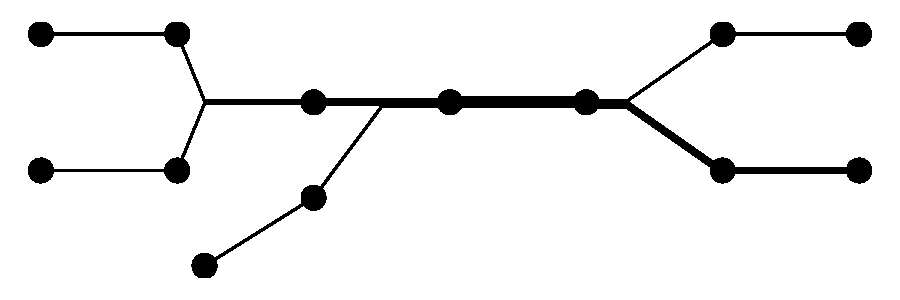
\includegraphics[width=0.95\textwidth]{figures/02_network_segments_2.pdf}
        \caption{GTFS-based road network}
        \label{fig:network_creation_2}
    \end{subfigure}
    \caption{Construction of a route network involves combining routes at nodes %
        (here we are using stops) which are connected by edges (roads). %
        In (a), the three unique routes, represented by different line types, clearly %
        overlap in several places. In (b) these have been merged, and the width of each line %
        represents how many routes use that link.}
    \label{fig:network_creation}
\end{figure}


\subsection{Realtime vehicle locations}
\label{sec:realtime_data}

GTFS \rt allows developers to query the current positions of vehicles
in the transit network.
The data consists of the time $t_k$ that the observation was made,
the GPS position of the vehicle, $\bY_k$, 
and some other information about the trip being serviced.
Vehicle positions are updated with a frequency of anywhere between 10~seconds and several minutes,
so there is often a lot of uncertainty about the trajectory
between two observations, particularly when there is one or more bus stop
or intersection between them.

Another complication with the Auckland Transport realtime feed is that
the buses are programmed to report their location when arriving at
bus stops and some major intersections.
Often these positions appear to be preemptive 
(i.e., the bus is almost there, but not quite),
and subsequent observations place the bus \emph{behind} the stop or intersection
(e.g., in a queue of traffic at traffic lights).
To handle this, we compute the approximate distance traveled, $\tilde x_k$,
of the vehicle by finding the nearest point on the path to the observation;
if this has decreased, the previous observation is rejected and the vehicle reverted
to its previous state.

